% ============================================================
% part2.tex —— 对应原 PDF 第 17-32 页
% 接 part1 末尾：问题（torch_compile）第 (a) 小问之后
% ============================================================

\textbf{交付物：}一张表格，比较你的编译版注意力模块与前文 \tm{pytorch\_attention} 问题中未编译版本的前向与反向传播耗时。

\begin{enumerate}[label=(\alph*), start=2]
  \item 接下来，在你的端到端基准测试脚本中编译整个 Transformer 模型。前向传播的性能有何变化？前向传播加反向传播以及优化器步骤合并起来的性能又如何？

  \textbf{交付物：}一张表格，比较你的原始（未编译）版本与编译后的 Transformer 模型。
\end{enumerate}

鉴于我们所看到的随序列长度变化的扩展行为，要处理长序列就需要显著的改进。即使使用 \tm{torch.compile}，当前实现在长序列长度下仍然存在非常糟糕的内存访问模式。为此，我们将编写 FlashAttention-2 的 Triton 实现，从而对内存的访问方式以及何时计算什么拥有大得多的控制权。

\subsubsection{示例：加权和}

为了介绍关于 Triton 你需要了解的内容以及它与 PyTorch 的互操作方式，我们将通过一个“加权和”（weighted sum）运算的示例核函数来讲解。更多上手 Triton 的资源请参阅 Triton 的官方教程。我们注意到，这些教程并未使用新的、便利的块指针（block pointer）抽象，下面我们将详细介绍它。

给定一个输入矩阵 $X$，我们将其各元素乘以一个按列的权重向量 $w$，然后对每一行求和，得到 $X$ 与 $w$ 的矩阵--向量乘积。我们先过一遍该运算的前向传播，然后再编写反向传播的 Triton 核函数。

\subsubsection*{前向传播}

我们核函数的前向传播就是下面这个广播内积。

\begin{lstlisting}[language=Python]
def weighted_sum(x, weight):
    # 这里假设 x 是 n 维张量，形状为 [..., D]，weight 是 1 维张量，形状为 [D]
    return (weight * x).sum(axis=-1)
\end{lstlisting}

在编写 Triton 核函数时，我们让每个程序实例（可能并行运行）计算 $x$ 的一个行分块（tile）的加权和，并把相应的标量输出写入输出张量。在 Triton 中，一个程序实例是运行同一程序的一块线程（block of threads），这些线程块可以在 GPU 上并行运行。我们不把张量本身作为参数传入，而是传入指向其首元素的指针，以及每个张量的步长（stride），步长告诉我们如何沿各个轴移动。

我们可以利用步长来加载与当前实例正在求和的 $x$ 行分块相对应的张量，并用程序 ID 来划分工作（即实例 $i$ 处理 $x$ 的第 $i$ 个行分块）。在这个简单的例子里，Triton 前向传播与 PyTorch 前向传播的主要区别在于需要进行指针运算以及显式的加载/存储。我们将使用块指针抽象（\tm{tl.make\_block\_ptr}）来大幅简化指针运算，不过这意味着需要做一些准备工作来构造块指针。

\begin{figure}[htbp]
\centering
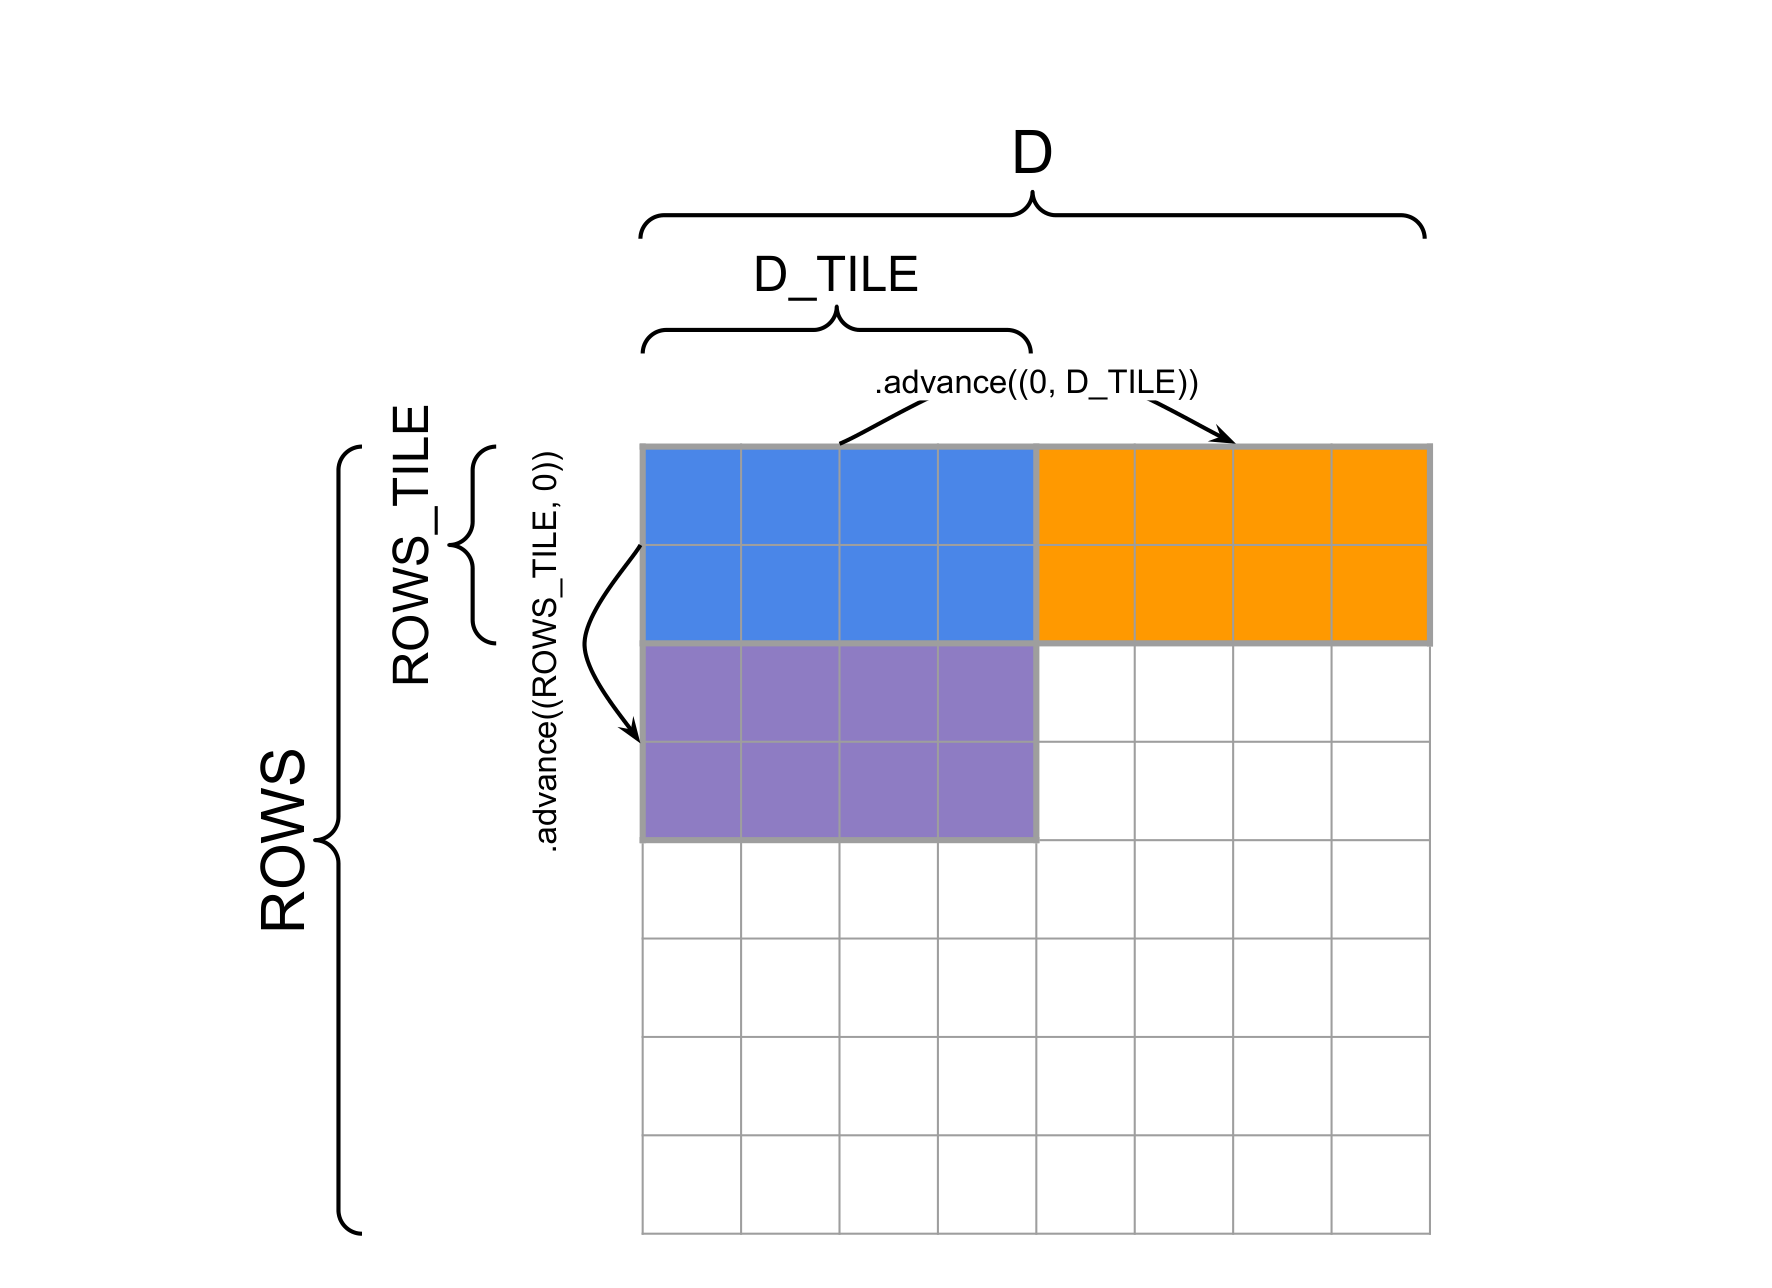
\includegraphics[width=0.62\textwidth]{figures/p18_fig2_crop.png}
\caption{加权和核函数示例（第 4.2.1 节）中分块的划分与块指针的推进}
\end{figure}

图 2 给出了分块以及块指针如何推进的示意图。上面的加权和函数如下所示：

\begin{lstlisting}[language=Python]
import triton
import triton.language as tl

@triton.jit
def weighted_sum_fwd(
    x_ptr, weight_ptr,  # 输入指针
    output_ptr,  # 输出指针
    x_stride_row, x_stride_dim,  # 步长告诉我们如何沿张量每个轴移动一个元素
    weight_stride_dim,  # 很可能是 1
    output_stride_row,  # 很可能是 1
    NUM_ROWS, D,
    ROWS_TILE_SIZE: tl.constexpr, D_TILE_SIZE: tl.constexpr,  # 分块形状必须在编译期已知
):
    # 每个实例将计算 x 的一个行分块的加权和。
    # `tl.program_id` 让我们能够知道自己正运行在哪个线程块中
    row_tile_idx = tl.program_id(0)
    # 块指针让我们可以从一块 N 维内存区域中进行选取，
    #  并移动我们选取的区域。
    # 块指针必须知道：
    # - 指向张量首元素的指针
    # - 张量的整体形状，以处理越界访问
    # - 每个维度的步长，以正确使用内存布局
    # - 起始块的 N 维坐标，即 "offsets"
    # - 每次加载/存储的分块形状
    # - 各维度在内存中从主要（major）到次要（minor）的顺序
    #    （= np.argsort(strides)），用于优化；>=Hopper 架构上的
    #    TMA 支持也需要它
    x_block_ptr = tl.make_block_ptr(
        x_ptr,
        shape=(NUM_ROWS, D,),
        strides=(x_stride_row, x_stride_dim),
        offsets=(row_tile_idx * ROWS_TILE_SIZE, 0),
        block_shape=(ROWS_TILE_SIZE, D_TILE_SIZE),
        order=(1, 0),
    )
    weight_block_ptr = tl.make_block_ptr(
        weight_ptr,
        shape=(D,),
        strides=(weight_stride_dim,),
        offsets=(0,),
        block_shape=(D_TILE_SIZE,),
        order=(0,),
    )
    output_block_ptr = tl.make_block_ptr(
        output_ptr,
        shape=(NUM_ROWS,),
        strides=(output_stride_row,),
        offsets=(row_tile_idx * ROWS_TILE_SIZE,),
        block_shape=(ROWS_TILE_SIZE,),
        order=(0,),
    )
    # 初始化一个待写入的缓冲区
    output = tl.zeros((ROWS_TILE_SIZE,), dtype=tl.float32)
    for i in range(tl.cdiv(D, D_TILE_SIZE)):
        # 加载当前的块指针
        # 由于 ROWS_TILE_SIZE 可能无法整除 NUM_ROWS，且 D_TILE_SIZE 可能无法整除 D，
        # 我们需要对两个维度都做边界检查
        row = tl.load(x_block_ptr, boundary_check=(0, 1), padding_option="zero")  # (ROWS_TILE_SIZE, D_TILE_SIZE)
        weight = tl.load(weight_block_ptr, boundary_check=(0,), padding_option="zero")  # (D_TILE_SIZE,)
        # 计算该行的加权和。
        output += tl.sum(row * weight[None, :], axis=1)
        # 把指针移动到下一个分块。
        # 这些是 (行, 列) 坐标增量
        x_block_ptr = x_block_ptr.advance((0, D_TILE_SIZE))  # 在最后一维上移动 D_TILE_SIZE
        weight_block_ptr = weight_block_ptr.advance((D_TILE_SIZE,))  # 移动 D_TILE_SIZE
    # 把输出写到输出块指针（每行一个标量）。
    # 由于 ROWS_TILE_SIZE 可能无法整除 NUM_ROWS，我们需要边界检查
    tl.store(output_block_ptr, output, boundary_check=(0,))
\end{lstlisting}

接下来，我们把这个核函数包装进一个 PyTorch Autograd 函数，使其能与 PyTorch 互操作（即以张量为输入、输出一个张量，并且之后在反向传播时也能与自动求导引擎协同工作）：

\begin{lstlisting}[language=Python]
class WeightedSumFunc(torch.autograd.Function):
    @staticmethod
    def forward(ctx, x, weight):
        # 缓存 x 和 weight 供反向传播使用：届时
        # 我们只会拿到关于输出张量的梯度，而
        # 需要计算关于 x 和 weight 的梯度。
        D, output_dims = x.shape[-1], x.shape[:-1]
        # 把输入张量重塑为 2 维
        input_shape = x.shape
        x = rearrange(x, "... d -> (...) d")
        ctx.save_for_backward(x, weight)
        assert len(weight.shape) == 1 and weight.shape[0] == D, "Dimension mismatch"
        assert x.is_cuda and weight.is_cuda, "Expected CUDA tensors"
        assert x.is_contiguous(), "Our pointer arithmetic will assume contiguous x"
        ctx.D_TILE_SIZE = triton.next_power_of_2(D) // 16  # 大约沿嵌入维度循环 16 次
        ctx.ROWS_TILE_SIZE = 16  # 每个线程一次处理 16 个批次元素
        ctx.input_shape = input_shape
        # 需要初始化一个空的结果张量。注意这些元素不一定是 0！
        y = torch.empty(output_dims, device=x.device)
        # 在 1 维网格中以 n 个实例启动我们的核函数。
        n_rows = y.numel()
        weighted_sum_fwd[(triton.cdiv(n_rows, ctx.ROWS_TILE_SIZE),)](
            x, weight,
            y,
            x.stride(0), x.stride(1),
            weight.stride(0),
            y.stride(0),
            NUM_ROWS=n_rows, D=D,
            ROWS_TILE_SIZE=ctx.ROWS_TILE_SIZE, D_TILE_SIZE=ctx.D_TILE_SIZE,
        )
        return y.view(input_shape[:-1])
\end{lstlisting}

注意，当我们以 \tm{weighted\_sum\_fwd[(triton.cdiv(n\_rows, ctx.ROWS\_TILE\_SIZE),)]} 调用 Triton 核函数时，我们通过传入元组 \tm{(triton.cdiv(n\_rows, ctx.ROWS\_TILE\_SIZE),)} 定义了一个所谓的线程块“启动网格”（launch grid）。随后，在核函数内部我们可以用 \tm{tl.program\_id(0)} 访问线程块索引。

\subsubsection*{反向传播}

由于我们定义了自己的核函数，我们也需要编写自己的反向函数。

在前向传播中，我们拿到层的输入，需要计算它的输出。而在反向传播中，回想一下，我们会拿到目标函数关于我们输出的梯度，需要计算关于每个输入的梯度。在我们的例子中，我们的运算以一个矩阵 $\boldsymbol{x} \in \mathbb{R}^{n\times h}$ 和一个权重向量 $\boldsymbol{w} \in \mathbb{R}^{h}$ 作为输入。为简洁起见，把我们的运算记为 $f(\boldsymbol{x}, \boldsymbol{w})$，其值域为 $\mathbb{R}^{n}$。那么，假设给定 $\nabla_{f(\boldsymbol{x},\boldsymbol{w})}\mathcal{L}$，即损失 $\mathcal{L}$ 关于该层输出的梯度，我们可以应用多元链式法则，得到关于 $\boldsymbol{x}$ 和 $\boldsymbol{w}$ 的梯度的如下表达式：

\begin{equation}
(\nabla_{\boldsymbol{x}} \mathcal{L})_{ij} = \sum_{k=1}^{n} \frac{\partial f(\boldsymbol{x}, \boldsymbol{w})_k}{\partial x_{ij}} \left( \nabla_{f(\boldsymbol{x},\boldsymbol{w})} \mathcal{L} \right)_{\!k} = w_j \cdot \left( \nabla_{f(\boldsymbol{x},\boldsymbol{w})} \mathcal{L} \right)_{\!i}
\end{equation}

\begin{equation}
(\nabla_{\boldsymbol{w}} \mathcal{L})_{j} = \sum_{i=1}^{n} \frac{\partial f(\boldsymbol{x}, \boldsymbol{w})_i}{\partial w_{j}} \left( \nabla_{f(\boldsymbol{x},\boldsymbol{w})} \mathcal{L} \right)_{\!i} = \sum_{i=1}^{n} x_{ij} \cdot \left( \nabla_{f(\boldsymbol{x},\boldsymbol{w})} \mathcal{L} \right)_{\!i}
\end{equation}

这为计算反向传播给出了一个简单的公式。要得到关于 $\boldsymbol{x}$ 的反向更新，我们应用式 (2)，取 $\boldsymbol{w}$ 与 $\nabla_{f(\boldsymbol{x},\boldsymbol{w})}\mathcal{L}$ 的外积。要计算关于 $\boldsymbol{w}$ 的反向更新（即 $(\nabla_{\boldsymbol{w}}\mathcal{L})_j$），我们必须把输入梯度乘以相应的输出行。

我们的反向传播核函数首先定义所有块指针，然后计算 $\nabla_{\boldsymbol{x}}\mathcal{L}$：

\begin{lstlisting}[language=Python]
@triton.jit
def weighted_sum_backward(
    x_ptr, weight_ptr,  # 输入
    grad_output_ptr,  # 梯度输入
    grad_x_ptr, partial_grad_weight_ptr,  # 梯度输出
    stride_xr, stride_xd,
    stride_wd,
    stride_gr,
    stride_gxr, stride_gxd,
    stride_gwb, stride_gwd,
    NUM_ROWS, D,
    ROWS_TILE_SIZE: tl.constexpr, D_TILE_SIZE: tl.constexpr,
):
    row_tile_idx = tl.program_id(0)
    n_row_tiles = tl.num_programs(0)
    # 输入
    grad_output_block_ptr = tl.make_block_ptr(
        grad_output_ptr,
        shape=(NUM_ROWS,), strides=(stride_gr,),
        offsets=(row_tile_idx * ROWS_TILE_SIZE,),
        block_shape=(ROWS_TILE_SIZE,),
        order=(0,),
    )
    x_block_ptr = tl.make_block_ptr(
        x_ptr,
        shape=(NUM_ROWS, D,), strides=(stride_xr, stride_xd),
        offsets=(row_tile_idx * ROWS_TILE_SIZE, 0),
        block_shape=(ROWS_TILE_SIZE, D_TILE_SIZE),
        order=(1, 0),
    )
    weight_block_ptr = tl.make_block_ptr(
        weight_ptr,
        shape=(D,), strides=(stride_wd,),
        offsets=(0,), block_shape=(D_TILE_SIZE,),
        order=(0,),
    )
    grad_x_block_ptr = tl.make_block_ptr(
        grad_x_ptr,
        shape=(NUM_ROWS, D,), strides=(stride_gxr, stride_gxd),
        offsets=(row_tile_idx * ROWS_TILE_SIZE, 0),
        block_shape=(ROWS_TILE_SIZE, D_TILE_SIZE),
        order=(1, 0),
    )
    partial_grad_weight_block_ptr = tl.make_block_ptr(
        partial_grad_weight_ptr,
        shape=(n_row_tiles, D,), strides=(stride_gwb, stride_gwd),
        offsets=(row_tile_idx, 0),
        block_shape=(1, D_TILE_SIZE),
        order=(1, 0),
    )
    for i in range(tl.cdiv(D, D_TILE_SIZE)):
        grad_output = tl.load(grad_output_block_ptr, boundary_check=(0,), padding_option="zero")  # (ROWS_TILE_SIZE,)
        # 用外积计算 grad_x
        weight = tl.load(weight_block_ptr, boundary_check=(0,), padding_option="zero")  # (D_TILE_SIZE,)
        grad_x_row = grad_output[:, None] * weight[None, :]
        tl.store(grad_x_block_ptr, grad_x_row, boundary_check=(0, 1))
        # 对 grad_weight 结果尽可能多地进行行归约
        row = tl.load(x_block_ptr, boundary_check=(0, 1), padding_option="zero")  # (ROWS_TILE_SIZE, D_TILE_SIZE)
        grad_weight_row = tl.sum(row * grad_output[:, None], axis=0, keep_dims=True)
        tl.store(partial_grad_weight_block_ptr, grad_weight_row, boundary_check=(1,))  # 在维度 0 上永远不会越界
        # 把指针沿 D 移动到下一个分块
        x_block_ptr = x_block_ptr.advance((0, D_TILE_SIZE))
        weight_block_ptr = weight_block_ptr.advance((D_TILE_SIZE,))
        partial_grad_weight_block_ptr = partial_grad_weight_block_ptr.advance((0, D_TILE_SIZE))
        grad_x_block_ptr = grad_x_block_ptr.advance((0, D_TILE_SIZE))
\end{lstlisting}

计算 $\nabla_{\boldsymbol{x}}$ 很简单，我们把结果写到输出张量相应的分块上即可。然而，计算 $\nabla_{\boldsymbol{w}}$ 稍微棘手一些。每个核函数实例负责 $x$ 的一个行分块，但我们现在需要沿 $x$ 的行求和。我们不直接在反向传播中做这个求和，而是约定 \tm{partial\_grad\_weight\_ptr} 指向一个 \tm{n\_row\_tiles} $\times$ $H$ 的矩阵，其中第一个维度只在 $x$ 的一个行分块内归约：我们在写入该张量之前，先在当前行分块内归约。在核函数之外，我们再用 \tm{torch.sum} 对 $\nabla_{\boldsymbol{w}}$ 做归约，把各个行分块的结果加起来。\footnote{当然，我们也可以为此专门编写自己的核函数。}

\tm{autograd.Function} 的最后一部分就相对简单了：

\begin{lstlisting}[language=Python]
class WeightedSumFunc(torch.autograd.Function):
    @staticmethod
    def forward(ctx, x, weight):
        # ...（定义见前文）
    @staticmethod
    def backward(ctx, grad_out):
        x, weight = ctx.saved_tensors
        ROWS_TILE_SIZE, D_TILE_SIZE = ctx.ROWS_TILE_SIZE, ctx.D_TILE_SIZE  # 它们不必相同
        n_rows, D = x.shape
        # 我们的策略是：每个线程块先写入一个部分和缓冲区，
        # 然后我们对该缓冲区做归约，得到最终梯度。
        partial_grad_weight = torch.empty((triton.cdiv(n_rows, ROWS_TILE_SIZE), D), device=x.device, dtype=x.dtype)
        grad_x = torch.empty_like(x)
        weighted_sum_backward[(triton.cdiv(n_rows, ROWS_TILE_SIZE),)](
            x, weight,
            grad_out,
            grad_x, partial_grad_weight,
            x.stride(0), x.stride(1),
            weight.stride(0),
            grad_out.stride(0),
            grad_x.stride(0), grad_x.stride(1),
            partial_grad_weight.stride(0), partial_grad_weight.stride(1),
            NUM_ROWS=n_rows, D=D,
            ROWS_TILE_SIZE=ROWS_TILE_SIZE, D_TILE_SIZE=D_TILE_SIZE,
        )
        grad_weight = partial_grad_weight.sum(axis=0)
        return grad_x, grad_weight
\end{lstlisting}

最后，我们现在可以得到一个用起来很像 \tm{torch.nn.functional} 中那些函数的函数：

\begin{lstlisting}[language=Python]
f_weightedsum = WeightedSumFunc.apply
\end{lstlisting}

现在，对两个 PyTorch 张量 $x$ 和 $w$ 调用 \tm{f\_weightedsum} 会得到如下形式的张量：

\begin{lstlisting}
tensor([ 90.8563, -93.6815, -80.8884,  ..., 103.4840, -21.4634, -24.0192],
       device='cuda:0', grad_fn=<WeightedSumFuncBackward>)
\end{lstlisting}

注意张量上附带的 \tm{grad\_fn}——它表明当这个张量出现在计算图中时，PyTorch 知道在反向传播时该调用什么。至此，我们完成了加权和运算的 Triton 实现。

\subsubsection{FlashAttention-2 前向传播}

你将用一个显著改进的、遵循 FlashAttention-2 [T. Dao, 2023] 的 Triton 实现来替换你的 PyTorch 注意力实现。FlashAttention-2 采用一些技巧按分块（tile）计算前向传播，从而获得高效的内存访问模式，并避免在全局内存中具体化完整的注意力矩阵。

在进入本节之前，我们强烈建议至少读一遍原始的 FlashAttention 论文 [T. Dao et al., 2022]，它会让你直观理解 FlashAttention 实现高效注意力的核心技术：以在线（online）方式跨分块计算 softmax（该技巧由 [M. Milakov et al., 2018] 提出）。我们还推荐阅读 H. He [4]，以便更直观地了解 GPU 实际上是如何执行 PyTorch 代码的。

\subsubsection*{理解朴素注意力的低效之处}

回想一下，注意力的前向传播（暂时忽略掩码）可以写为：
\begin{equation}
\boldsymbol{S} = \boldsymbol{Q}\boldsymbol{K}^{\top} / \sqrt{d}
\end{equation}
\begin{equation}
P_{ij} = \mathrm{softmax}_j(\boldsymbol{S})_{ij}
\end{equation}
\begin{equation}
\boldsymbol{O} = \boldsymbol{P}\boldsymbol{V}
\end{equation}

标准反向传播为
\begin{equation}
\boldsymbol{dV} = \boldsymbol{P}^{\top} \boldsymbol{dO}
\end{equation}
\begin{equation}
\boldsymbol{dP} = \boldsymbol{dO}\boldsymbol{V}^{\top}
\end{equation}
\begin{equation}
\boldsymbol{dS}_i = \mathrm{dsoftmax}(\boldsymbol{dP}_i) = \left(\mathrm{diag}(\boldsymbol{P}_i) - \boldsymbol{P}_i \boldsymbol{P}_i^{\top}\right) \boldsymbol{dP}_i
\end{equation}
\begin{equation}
\boldsymbol{dQ} = \boldsymbol{dS}\boldsymbol{K} / \sqrt{d}
\end{equation}
\begin{equation}
\boldsymbol{dK} = \boldsymbol{dS}^{\top} \boldsymbol{Q} / \sqrt{d}
\end{equation}

正如你所见，反向传播依赖前向传播中一些非常大的激活值。例如，式 (7) 中计算 $\boldsymbol{dV}$ 需要 $\boldsymbol{P}$，即形状为 \tm{(batch\_size, n\_heads, seq\_len, seq\_len)} 的注意力分数——这个激活矩阵的大小随序列长度\emph{平方级}增长，这正好解释了我们之前在大序列长度下对注意力做基准测试时遇到的内存问题。在朴素注意力的前向与反向传播过程中，为在片上 SRAM 与 GPU HBM 之间搬运 $\boldsymbol{P}$ 及其他大型激活值，我们要付出可观的内存 IO 代价。标准实现中存在多次这样的传输：例如，标准的反向传播实现会在式 (7) 和式 (9) 的计算中都从 HBM 读取 $\boldsymbol{P}$。

FlashAttention 的主要目标是避免把注意力矩阵在 HBM 中读入写出，以降低 IO 和峰值内存开销。我们通过三种技术来做到这一点：分块（tiling）、重计算（recomputation）和算子融合（operator fusion）。

\subsubsection*{分块}

为了避免在 HBM 中读写注意力矩阵，我们在无法一次性访问整个输入的情况下计算 softmax 归约。具体而言，我们重构注意力计算，把输入切分成若干分块，并对输入分块进行多趟处理，从而增量式地执行 softmax 归约。

\subsubsection*{重计算}

我们避免在 HBM 中存储形状为 \tm{(batch\_size, n\_heads, seq\_len, seq\_len)} 的大型中间注意力矩阵。作为替代，我们在 HBM 中保存一些“激活检查点”，然后在反向传播期间重计算前向传播的一部分，以得到计算梯度所需的其他激活值。FlashAttention-2 还会保存注意力分数的 logsumexp 值 $L$，用于简化反向传播的计算。$L$ 的表达式为：
\begin{equation}
L_i = \log\left(\sum_j \exp(S_{ij})\right)
\end{equation}

在我们的最终核函数中，我们会以在线的方式计算它，但最终结果应当相同。结合分块与重计算，我们的内存 IO 和峰值内存占用不再依赖于 $\mathrm{sequence\_length}^2$，因此我们可以使用更大的序列长度。

\subsubsection*{算子融合}

最后，我们把所有运算放进单个核函数中执行，从而避免对注意力矩阵和其他中间激活值的反复内存 IO——这称为算子融合（operator fusion）或核函数融合（kernel fusion）。我们将为前向传播编写一个单独的 Triton 核函数，在 HBM 与 SRAM 之间仅进行有限数据传输的情况下完成注意力涉及的全部运算。算子融合在一定程度上得益于重计算：这样我们就可以省去为保存每个中间激活值而付出的内存 IO。

想要对这些技巧有更多直观理解，可以参阅 FlashAttention 论文 [T. Dao et al., 2022; T. Dao, 2023]。

\subsubsection*{带重计算的反向传播}

利用 $L$，我们可以进行恰当的重计算并高效地计算反向传播。在开始反向传播之前，我们先在全局内存中预计算 $D = \mathrm{rowsum}(\boldsymbol{O} \circ \boldsymbol{dO})$（其中 $\circ$ 表示逐元素相乘），它等于 $\mathrm{rowsum}(\boldsymbol{P} \circ \boldsymbol{dP})$，因为 $\boldsymbol{P}\boldsymbol{dP}^{\top} = \boldsymbol{P}(\boldsymbol{dO}\boldsymbol{V}^{\top})^{\top} = (\boldsymbol{P}\boldsymbol{V})\boldsymbol{dO}^{\top} = \boldsymbol{O}\boldsymbol{dO}^{\top}$（且对任意矩阵 $\boldsymbol{A}$、$\boldsymbol{B}$ 有 $\mathrm{rowsum}(\boldsymbol{A} \circ \boldsymbol{B}) = \mathrm{diag}(\boldsymbol{A}\boldsymbol{B}^{\top})$）。有了 $L$ 和 $D$ 这两个向量，反向传播的计算就不再需要 softmax。完整的反向传播计算现在是：
\begin{equation}
\boldsymbol{S} = \boldsymbol{Q}\boldsymbol{K}^{\top} / \sqrt{d}
\end{equation}
\begin{equation}
P_{ij} = \exp(S_{ij} - L_i)
\end{equation}
\begin{equation}
\boldsymbol{dV} = \boldsymbol{P}^{\top} \boldsymbol{dO}
\end{equation}
\begin{equation}
\boldsymbol{dP} = \boldsymbol{dO}\boldsymbol{V}^{\top}
\end{equation}
\begin{equation}
dS_{ij} = P_{ij}\left(dP_{ij} - D_i\right)
\end{equation}
\begin{equation}
\boldsymbol{dQ} = \boldsymbol{dS}\boldsymbol{K} / \sqrt{d}
\end{equation}
\begin{equation}
\boldsymbol{dK} = \boldsymbol{dS}^{\top} \boldsymbol{Q} / \sqrt{d}
\end{equation}

可以看到，这一串运算不再要求我们在前向传播期间把注意力分数 $\boldsymbol{P}$ 存入 HBM——我们在式 (13) 和式 (14) 中从激活值 $\boldsymbol{Q}$、$\boldsymbol{K}$ 和 $L$ 重计算它们。

\subsubsection*{FlashAttention 前向传播的细节}

现在我们对 FlashAttention-2 使用的技巧有了高层认识，接下来深入了解你将要实现的 FA2 前向传播核函数的细节。为了避免在 HBM 中读写注意力矩阵，我们希望使用分块，也就是说，独立于其他分块地计算输出的每一个分块。这要求我们能够对 $\boldsymbol{P}$ 分块计算，理想情况下在两个维度（query 和 key）上都分块。

然而，当我们对 $\boldsymbol{S}$ 应用 softmax 时，需要对 $\boldsymbol{S}$ 的整行做归约来计算 softmax 的分母，这意味着我们无法直接分块计算 $\boldsymbol{P}$。FlashAttention-2 使用在线 softmax（online softmax）解决了这个问题。在下文中，我们用下标 $i$ 表示当前 query 分块，用上标 $(j)$ 表示当前 key 分块。沿 query 维度的分块大小为 $B_q$，沿 key 维度的分块大小为 $B_k$。我们不会沿隐藏维度 $d$ 分块。

我们还维护一些按行运算的运行值 $\boldsymbol{m}_i^{(j)} \in \mathbb{R}^{B_q}$ 和 $\boldsymbol{l}_i^{(j)} \in \mathbb{R}^{B_q}$。按行的 $\boldsymbol{m}_i^{(j)}$ 值是一个运行最大值，记录它使我们能够以数值稳定的方式计算 softmax（回忆一下作业 1 中 softmax 实现里的这个技巧）。当 $j$ 增大时（即遇到 $\boldsymbol{S}$ 的新行分块），我们会更新 $\boldsymbol{m}_i^{(j)}$。利用这个运行最大值，我们可以把未归一化的 softmax 值（分子）计算为 $\tilde{\boldsymbol{P}}_i^{(j)} = \exp(\boldsymbol{S}_{ij} - \boldsymbol{m}_i^{(j)})$。$\boldsymbol{l}_i^{(j)}$ 是 softmax 分母的运行代理值，它将用未归一化的 softmax 值更新为 $\boldsymbol{l}_i^{(j)} = \exp(\boldsymbol{m}_i^{(j-1)} - \boldsymbol{m}_i^{(j)}) \cdot \boldsymbol{l}_i^{(j-1)} + \mathrm{rowsum}(\tilde{\boldsymbol{P}}_i^{(j)})$。最终写出输出时，我们需要用 $\boldsymbol{l}_i^{(T_k)}$（处理完全部 key 分块后 $\boldsymbol{l}_i^{(j)}$ 的最终值）完成归一化。算法 1 展示了 GPU 上的前向传播。

\begin{center}
\textbf{算法 1：FlashAttention-2 的前向传播}
\end{center}

\begin{enumerate}[label=\arabic*., leftmargin=2.2em, itemsep=1pt, parsep=0pt]
  \item \textbf{需要：}$\boldsymbol{Q} \in \mathbb{R}^{N_q \times d}$，$\boldsymbol{K}, \boldsymbol{V} \in \mathbb{R}^{N_k \times d}$，分块大小 $B_q$、$B_k$
  \item 把 $\boldsymbol{Q}$ 划分为 $T_q = \lceil \frac{N_q}{B_q} \rceil$ 个大小为 $B_q \times d$ 的分块 $\boldsymbol{Q}_1, \dots, \boldsymbol{Q}_{T_q}$
  \item 把 $\boldsymbol{K}, \boldsymbol{V}$ 划分为 $T_k = \lceil \frac{N_k}{B_k} \rceil$ 个大小为 $B_k \times d$ 的分块 $\boldsymbol{K}^{(1)}, \dots, \boldsymbol{K}^{(T_k)}$ 与 $\boldsymbol{V}^{(1)}, \dots, \boldsymbol{V}^{(T_k)}$
  \item \textbf{for} $i = 1, \dots, T_q$ \textbf{do}
  \item \hspace*{1.6em}从全局内存加载 $\boldsymbol{Q}_i$
  \item \hspace*{1.6em}初始化 $\boldsymbol{O}_i^{(0)} = \boldsymbol{0} \in \mathbb{R}^{B_q \times d}$，$\boldsymbol{l}_i^{(0)} = 0 \in \mathbb{R}^{B_q}$，$\boldsymbol{m}_i^{(0)} = -\infty \in \mathbb{R}^{B_q}$
  \item \hspace*{1.6em}\textbf{for} $j = 1, \dots, T_k$ \textbf{do}
  \item \hspace*{3.2em}从全局内存加载 $\boldsymbol{K}^{(j)}, \boldsymbol{V}^{(j)}$
  \item \hspace*{3.2em}计算 pre-softmax 注意力分数分块 $\boldsymbol{S}_i^{(j)} = \frac{\boldsymbol{Q}_i (\boldsymbol{K}^{(j)})^{\top}}{\sqrt{d}} \in \mathbb{R}^{B_q \times B_k}$
  \item \hspace*{3.2em}计算 $\boldsymbol{m}_i^{(j)} = \max\left(\boldsymbol{m}_i^{(j-1)}, \mathrm{rowmax}(\boldsymbol{S}_i^{(j)})\right) \in \mathbb{R}^{B_q}$
  \item \hspace*{3.2em}计算 $\tilde{\boldsymbol{P}}_i^{(j)} = \exp\left(\boldsymbol{S}_i^{(j)} - \boldsymbol{m}_i^{(j)}\right) \in \mathbb{R}^{B_q \times B_k}$
  \item \hspace*{3.2em}计算 $\boldsymbol{l}_i^{(j)} = \exp\left(\boldsymbol{m}_i^{(j-1)} - \boldsymbol{m}_i^{(j)}\right) \boldsymbol{l}_i^{(j-1)} + \mathrm{rowsum}\left(\tilde{\boldsymbol{P}}_i^{(j)}\right) \in \mathbb{R}^{B_q}$
  \item \hspace*{3.2em}计算 $\boldsymbol{O}_i^{(j)} = \mathrm{diag}\left(\exp\left(\boldsymbol{m}_i^{(j-1)} - \boldsymbol{m}_i^{(j)}\right)\right) \boldsymbol{O}_i^{(j-1)} + \tilde{\boldsymbol{P}}_i^{(j)} \boldsymbol{V}^{(j)}$
  \item \hspace*{1.6em}\textbf{end for}
  \item \hspace*{1.6em}计算 $\boldsymbol{O}_i = \mathrm{diag}\left(\boldsymbol{l}_i^{(T_k)}\right)^{-1} \boldsymbol{O}_i^{(T_k)}$
  \item \hspace*{1.6em}计算 $L_i = \boldsymbol{m}_i^{(T_k)} + \log\left(\boldsymbol{l}_i^{(T_k)}\right)$
  \item \hspace*{1.6em}把 $\boldsymbol{O}_i$ 作为 $\boldsymbol{O}$ 的第 $i$ 个分块写入全局内存。
  \item \hspace*{1.6em}把 $L_i$ 作为 $L$ 的第 $i$ 个分块写入全局内存。
  \item \textbf{end for}
  \item 返回输出 $\boldsymbol{O}$ 与 logsumexp $L$。
\end{enumerate}

在开始用 Triton 实现前向传播之前，我们在这里汇总一些编写 Triton 核函数的通用技巧与窍门。

\subsubsection*{Triton 技巧与窍门}

\begin{itemize}
  \item 你可以在 Triton 中使用 \tm{tl.device\_print} 打印语句来调试：\\ {\footnotesize\url{https://triton-lang.org/main/python-api/generated/triton.language.device_print.html}}。还有一个设置 \tm{TRITON\_INTERPRET=1}，可以在 CPU 上运行 Triton 解释器，不过我们发现它 bug 不少。
  \item 定义块指针时，务必确保它们的偏移量（offsets）正确，并且块偏移乘上了相应的分块大小。
  \item 线程块的启动网格通过如下方式设置：
\begin{lstlisting}
kernel_fn[(launch_grid_d1, launch_grid_d2, ...)](...arguments...)
\end{lstlisting}
  即在 \tm{torch.autograd.Function} 子类的方法中这样调用，正如我们在加权和示例中看到的那样。
  \item 用 \tm{tl.dot} 执行矩阵乘法。
  \item 要推进块指针，使用 \tm{*\_block\_ptr = *\_block\_ptr.advance(...)}。
\end{itemize}

\subsubsection*{问题（\tm{flash\_forward}）：FlashAttention-2 前向传播（15 分）}

\begin{enumerate}[label=(\alph*)]
  \item 编写一个纯 PyTorch（不用 Triton）的 \tm{autograd.Function} 来实现 FlashAttention-2 前向传播。它会比常规的 PyTorch 实现慢很多，但能帮助你调试 Triton 核函数。

  你的实现应接受输入 $\boldsymbol{Q}$、$\boldsymbol{K}$、$\boldsymbol{V}$ 以及一个标志 \tm{is\_causal}，并产生输出 $\boldsymbol{O}$ 和 logsumexp 值 $L$。本题中你可以忽略 \tm{is\_causal} 标志。\tm{autograd.Function} 的 forward 随后应为反向传播保存 $L$、$\boldsymbol{Q}$、$\boldsymbol{K}$、$\boldsymbol{V}$、$\boldsymbol{O}$，并返回 $\boldsymbol{O}$。记住，\tm{autograd.Function} 的 forward 方法的实现总是以上下文（context）作为第一个参数。任何 \tm{autograd.Function} 类都需要实现一个 backward 方法，但现在你可以让它直接抛出 \tm{NotImplementedError}。如果你需要对比的对象，可以在 PyTorch 中实现式 (4) 到式 (6) 以及式 (12)，并比较你的输出。

  接口为 \tm{def forward(ctx, Q, K, V, is\_causal=False)}。分块大小自行确定，但要确保至少为 $16 \times 16$。我们测试你的代码时使用的维度总是 2 的幂且至少为 16，所以你不必担心越界访问。

  \textbf{交付物：}一个实现了 FlashAttention-2 前向传播的 \tm{torch.autograd.Function} 子类。要测试你的代码，实现 \tm{[adapters.get\_flashattention\_autograd\_function\_pytorch]}。然后运行 \tm{uv run pytest -k test\_flash\_forward\_pass\_pytorch}，确保你的实现通过测试。

  \item 按照算法 1，为 FlashAttention-2 的前向传播编写一个 Triton 核函数。然后编写另一个 \tm{torch.autograd.Function} 子类，让它在 forward 中调用这个（融合的）核函数，而不是在 PyTorch 中计算结果。几个针对本题的提示：
  \begin{itemize}
    \item 调试时，建议把你执行的每个 Triton 运算的结果与你在第 (a) 小问中编写的分块 PyTorch 实现进行比较。
    \item 你的启动网格应设为 $(T_q, \text{batch\_size})$，也就是说，每个 Triton 程序实例只加载单个 batch 索引的元素，并且只对 $\boldsymbol{Q}$、$\boldsymbol{O}$ 和 $L$ 的单个 query 分块进行读/写。
    \item 核函数应该只有一个循环，迭代 key 分块 $1 \le j \le T_k$。
    \item 在循环末尾推进块指针。
    \item 使用下面的函数声明（借助我们给你的块指针，你应该能推断出其余指针的设置）：
  \end{itemize}

\begin{lstlisting}[language=Python]
@triton.jit
def flash_fwd_kernel(
    Q_ptr, K_ptr, V_ptr,
    O_ptr, L_ptr,
    stride_qb, stride_qq, stride_qd,
    stride_kb, stride_kk, stride_kd,
    stride_vb, stride_vk, stride_vd,
    stride_ob, stride_oq, stride_od,
    stride_lb, stride_lq,
    N_QUERIES, N_KEYS,
    scale,
    D: tl.constexpr,
    Q_TILE_SIZE: tl.constexpr,
    K_TILE_SIZE: tl.constexpr,
):
    # 程序索引
    query_tile_index = tl.program_id(0)
    batch_index = tl.program_id(1)
    # 用对应的批次索引乘以每个张量的批次步长，来偏移各个指针
    Q_block_ptr = tl.make_block_ptr(
        Q_ptr + batch_index * stride_qb,
        shape=(N_QUERIES, D),
        strides=(stride_qq, stride_qd),
        offsets=(query_tile_index * Q_TILE_SIZE, 0),
        block_shape=(Q_TILE_SIZE, D),
        order=(1, 0),
    )
    ...
\end{lstlisting}

  其中 \tm{scale} 为 $1/\sqrt{d}$，\tm{Q\_TILE\_SIZE} 和 \tm{K\_TILE\_SIZE} 分别是 $B_q$ 和 $B_k$。你稍后可以调整它们。

  下面这些附加准则可以帮助你避免精度问题：
  \begin{itemize}
    \item 片上缓冲区（$\boldsymbol{O}_i$、$\boldsymbol{l}$、$\boldsymbol{m}$）的 dtype 应为 \tm{tl.float32}。如果你在向一个输出缓冲区累加，请使用 acc 参数（\tm{acc = tl.dot(..., acc=acc)}）。
    \item 在相乘之前，把 $\tilde{\boldsymbol{P}}_i^{(j)}$ 转换为 $\boldsymbol{V}^{(j)}$ 的 dtype；在把 $\boldsymbol{O}_i$ 写入全局内存之前，把它转换为合适的 dtype。类型转换用 \tm{tensor.to} 完成。你可以用 \tm{tensor.dtype} 获取张量的 dtype，用 \tm{*\_block\_ptr.type.element\_ty} 获取块指针/指针的 dtype。
  \end{itemize}

  \textbf{交付物：}一个 \tm{torch.autograd.Function} 子类，它使用你的 Triton 核函数实现 FlashAttention-2 前向传播。实现 \tm{[adapters.get\_flash\_autograd\_function\_triton]}。然后运行 \tm{uv run pytest -k test\_flash\_forward\_pass\_triton}，确保你的实现通过测试。

  \item 在你的 \tm{autograd.Function} 实现中，把一个标志作为最后一个参数加入，用于因果掩码（causal masking）。它应是一个布尔标志，设为 \tm{True} 时启用用于因果掩码的索引比较。你的 Triton 核函数应有对应的额外参数 \tm{is\_causal: tl.constexpr}（这是必需的类型标注）。在 Triton 中，为 query 和 key 构造合适的索引向量，并比较它们以形成大小为 $B_q \times B_k$ 的方形掩码。对于被掩码掉的元素，给注意力分数矩阵 $\boldsymbol{S}_i^{(j)}$ 的相应元素加上常数值 $-1e6$。务必用 \tm{ctx.is\_causal = is\_causal} 把掩码标志保存下来供反向传播使用。

  \textbf{交付物：}为你的 \tm{torch.autograd.Function} 子类添加一个额外的标志，使用你的 Triton 核函数实现带因果掩码的 FlashAttention-2 前向传播。确保该标志是可选的且默认为 \tm{False}，这样之前的测试仍能通过。
\end{enumerate}

\subsubsection*{用重计算实现反向传播}

注意，与式 (7) 到式 (11) 中的标准反向传播不同，我们可以利用重计算来避免式 (13) 到式 (19) 所示反向传播中的 softmax 运算。这意味着我们可以用一个简单的（trivial）核函数来计算反向传播，不需要任何在线技巧。因此在这一部分，你可以通过对一个常规 PyTorch 函数（非 Triton）调用 \tm{torch.compile} 来实现反向传播。

\subsubsection*{问题（\tm{flash\_backward}）：FlashAttention-2 反向传播（5 分）}

使用 PyTorch（非 Triton）和 \tm{torch.compile} 为你的 FlashAttention-2 \tm{autograd.Function} 实现反向传播。你的实现应接受 $\boldsymbol{Q}$、$\boldsymbol{K}$、$\boldsymbol{V}$、$\boldsymbol{O}$、$\boldsymbol{dO}$ 和 $L$ 张量作为输入，并返回 $\boldsymbol{dQ}$、$\boldsymbol{dK}$ 和 $\boldsymbol{dV}$。记得计算并使用 $D$ 向量。你可以按照式 (13) 到式 (19) 的计算来实现。

\textbf{交付物：}要测试你的实现，运行 \tm{uv run pytest -k test\_flash\_backward}。

现在，让我们把你的（部分）Triton 版 FlashAttention-2 实现与你的常规 Attention 的 PyTorch 实现进行性能比较。

\subsubsection*{问题（\tm{flash\_benchmarking}）：FlashAttention-2 基准测试（5 分）}

\begin{enumerate}[label=(\alph*)]
  \item 使用 \tm{triton.testing.do\_bench} 编写一个基准测试脚本，把你（部分）Triton 版 FlashAttention-2 的前向和反向传播性能与常规 PyTorch 实现（即不使用 FlashAttention）进行比较。

  具体而言，你要报告一张表格，其中包含你的 Triton 实现与 PyTorch 实现各自的前向、反向以及端到端前向--反向传播的延迟。在开始基准测试之前，随机生成一切必要的输入，并在单块 B200 上运行基准测试。始终使用批量大小 1 和因果掩码。遍历如下设定的笛卡尔积：序列长度取从 128 到 65536 的各种 2 的幂，嵌入维度大小取从 16 到 128 的各种 2 的幂，精度取 \tm{torch.bfloat16} 和 \tm{torch.float32}。你可能需要根据输入大小调整分块大小。

  \textbf{交付物：}一张结果表格，按上述设定比较你的 FlashAttention-2 实现与 PyTorch 实现，报告前向、反向和端到端延迟。
\end{enumerate}

\subsubsection{可选：Triton 反向传播}

如果你有兴趣获得更多 Triton 练习，和/或想提交一个快速的成绩榜（leaderboard）结果，我们在下面提供可以用 Triton 实现的分块 FlashAttention-2 反向传播。算法 2 展示了在 Triton 中应当如何实现 FlashAttention-2 的反向传播。这里的一个关键技巧是把 $\boldsymbol{P}$ 计算两次：一次用于 $\boldsymbol{dQ}$，再一次用于 $\boldsymbol{dK}$ 和 $\boldsymbol{dV}$。这让我们无需跨线程块同步，从而可以避免缓慢的原子操作（atomics）。

\begin{center}
\textbf{算法 2：分块的 FlashAttention-2 反向传播}
\end{center}

\begin{enumerate}[label=\arabic*., leftmargin=2.2em, itemsep=1pt, parsep=0pt]
  \item \textbf{需要：}$\boldsymbol{Q}, \boldsymbol{O}, \boldsymbol{dO} \in \mathbb{R}^{N_q \times d}$，$\boldsymbol{K}, \boldsymbol{V} \in \mathbb{R}^{N_k \times d}$，$L \in \mathbb{R}^{N_q}$，分块大小 $B_q$、$B_k$
  \item 计算 $D = \mathrm{rowsum}(\boldsymbol{O} \circ \boldsymbol{dO}) \in \mathbb{R}^{N_q}$
  \item 把 $\boldsymbol{Q}, \boldsymbol{O}, \boldsymbol{dO}$ 划分为 $T_q = \lceil \frac{N_q}{B_q} \rceil$ 个分块 $\boldsymbol{Q}_1, \dots, \boldsymbol{Q}_{T_q}$、$\boldsymbol{O}_1, \dots, \boldsymbol{O}_{T_q}$、$\boldsymbol{dO}_1, \dots, \boldsymbol{dO}_{T_q}$，每个大小为 $B_q \times d$
  \item 把 $\boldsymbol{K}, \boldsymbol{V}$ 划分为 $T_k = \lceil \frac{N_k}{B_k} \rceil$ 个分块 $\boldsymbol{K}^{(1)}, \dots, \boldsymbol{K}^{(T_k)}$ 与 $\boldsymbol{V}^{(1)}, \dots, \boldsymbol{V}^{(T_k)}$，每个大小为 $B_k \times d$
  \item 把 $L, D$ 划分为 $T_q$ 个分块 $L_1, \dots, L_{T_q}$ 与 $D_1, \dots, D_{T_q}$，每个大小为 $B_q$
  \item \textbf{for} $j = 1, \dots, T_k$ \textbf{do}
  \item \hspace*{1.6em}从全局内存加载 $\boldsymbol{K}^{(j)}, \boldsymbol{V}^{(j)}$
  \item \hspace*{1.6em}初始化 $\boldsymbol{dK}_0^{(j)} = \boldsymbol{dV}_0^{(j)} = \boldsymbol{0} \in \mathbb{R}^{B_k \times d}$
  \item \hspace*{1.6em}\textbf{for} $i = 1, \dots, T_q$ \textbf{do}
  \item \hspace*{3.2em}从全局内存加载 $\boldsymbol{Q}_i, \boldsymbol{dO}_i$
  \item \hspace*{3.2em}计算注意力分数分块 $\boldsymbol{S}_i^{(j)} = \frac{\boldsymbol{Q}_i (\boldsymbol{K}^{(j)})^{\top}}{\sqrt{d}} \in \mathbb{R}^{B_q \times B_k}$
  \item \hspace*{3.2em}计算注意力概率 $\boldsymbol{P}_i^{(j)} = \exp\left(\boldsymbol{S}_i^{(j)} - L_i\right) \in \mathbb{R}^{B_q \times B_k}$
  \item \hspace*{3.2em}计算 $\boldsymbol{dV}_i^{(j)} = \boldsymbol{dV}_{i-1}^{(j)} + \left(\boldsymbol{P}_i^{(j)}\right)^{\top} \boldsymbol{dO}_i \in \mathbb{R}^{B_k \times d}$
  \item \hspace*{3.2em}计算 $\boldsymbol{dP}_i^{(j)} = \boldsymbol{dO}_i \left(\boldsymbol{V}^{(j)}\right)^{\top} \in \mathbb{R}^{B_q \times B_k}$
  \item \hspace*{3.2em}计算 $\boldsymbol{dS}_i^{(j)} = \boldsymbol{P}_i^{(j)} \circ \left(\boldsymbol{dP}_i^{(j)} - D_i\right) \in \mathbb{R}^{B_q \times B_k}$
  \item \hspace*{3.2em}计算 $\boldsymbol{dK}_i^{(j)} = \boldsymbol{dK}_{i-1}^{(j)} + \left(\boldsymbol{dS}_i^{(j)}\right)^{\top} \boldsymbol{Q}_i / \sqrt{d} \in \mathbb{R}^{B_k \times d}$
  \item \hspace*{1.6em}\textbf{end for}
  \item \hspace*{1.6em}把 $\boldsymbol{dK}_{T_q}^{(j)}$ 和 $\boldsymbol{dV}_{T_q}^{(j)}$ 写入全局内存，作为 $\boldsymbol{dK}$ 和 $\boldsymbol{dV}$ 的第 $j$ 个分块。
  \item \textbf{end for}
  \item \textbf{for} $i = 1, \dots, T_q$ \textbf{do}
  \item \hspace*{1.6em}从全局内存加载 $\boldsymbol{Q}_i, \boldsymbol{dO}_i$
  \item \hspace*{1.6em}初始化 $\boldsymbol{dQ}_i^{(0)} = \boldsymbol{0} \in \mathbb{R}^{B_q \times d}$
  \item \hspace*{1.6em}\textbf{for} $j = 1, \dots, T_k$ \textbf{do}
  \item \hspace*{3.2em}从全局内存加载 $\boldsymbol{K}^{(j)}, \boldsymbol{V}^{(j)}$
  \item \hspace*{3.2em}计算注意力分数分块 $\boldsymbol{S}_i^{(j)} = \frac{\boldsymbol{Q}_i (\boldsymbol{K}^{(j)})^{\top}}{\sqrt{d}} \in \mathbb{R}^{B_q \times B_k}$
  \item \hspace*{3.2em}计算注意力概率 $\boldsymbol{P}_i^{(j)} = \exp\left(\boldsymbol{S}_i^{(j)} - L_i\right) \in \mathbb{R}^{B_q \times B_k}$
  \item \hspace*{3.2em}计算 $\boldsymbol{dP}_i^{(j)} = \boldsymbol{dO}_i \left(\boldsymbol{V}^{(j)}\right)^{\top} \in \mathbb{R}^{B_q \times B_k}$
  \item \hspace*{3.2em}计算 $\boldsymbol{dS}_i^{(j)} = \boldsymbol{P}_i^{(j)} \circ \left(\boldsymbol{dP}_i^{(j)} - D_i\right) \in \mathbb{R}^{B_q \times B_k}$
  \item \hspace*{3.2em}计算 $\boldsymbol{dQ}_i^{(j)} = \boldsymbol{dQ}_i^{(j-1)} + \boldsymbol{dS}_i^{(j)} \boldsymbol{K}^{(j)} / \sqrt{d} \in \mathbb{R}^{B_q \times d}$
  \item \hspace*{1.6em}\textbf{end for}
  \item \hspace*{1.6em}把 $\boldsymbol{dQ}_i^{(T_k)}$ 写入全局内存，作为 $\boldsymbol{dQ}$ 的第 $i$ 个分块。
  \item \textbf{end for}
  \item 返回 $\boldsymbol{dQ}, \boldsymbol{dK}, \boldsymbol{dV}$。
\end{enumerate}

\section{分布式数据并行训练}

在本作业的下一部分，我们将探索使用多 GPU 训练语言模型的方法，重点是数据并行（data parallelism）。我们先从 PyTorch 分布式通信的入门讲解开始。然后，我们将研究分布式数据并行训练的一种朴素实现，接着实现并基准测试各种提升通信效率的改进。

\subsection{PyTorch 单节点分布式通信}

我们先来看一个简单的 PyTorch 分布式应用，它的目标是生成四个随机整数张量并计算它们的和。

在下面的分布式情形中，我们将派生（spawn）四个工作进程，每个进程生成一个随机整数张量。为了跨工作进程对这些张量求和，我们将调用 all-reduce 集合通信（collective communication）操作，它会把每个进程上的原数据张量替换为 all-reduce 的结果（即总和）。

现在我们来看代码。

\begin{lstlisting}[language=Python]
import os
import torch
import torch.distributed as dist
import torch.multiprocessing as mp

def setup(rank, world_size):
    os.environ["MASTER_ADDR"] = "localhost"
    os.environ["MASTER_PORT"] = "29500"
    dist.init_process_group("gloo", rank=rank, world_size=world_size)

def distributed_demo(rank, world_size):
    setup(rank, world_size)
    data = torch.randint(0, 10, (3,))
    print(f"rank {rank} data (before all-reduce): {data}")
    dist.all_reduce(data, async_op=False)
    print(f"rank {rank} data (after all-reduce): {data}")

if __name__ == "__main__":
    world_size = 4
    mp.spawn(fn=distributed_demo, args=(world_size, ), nprocs=world_size, join=True)
\end{lstlisting}

运行上面的脚本之后，我们得到如下输出。正如预期，每个工作进程最初持有不同的数据张量。all-reduce 操作把所有工作进程的张量求和之后，每个工作进程上的数据被就地修改为 all-reduce 的结果。\footnote{如果你多次运行这个脚本，会注意到输出的打印顺序是不确定的。由于这个应用运行在分布式环境中，我们无法控制命令执行的确切顺序——我们唯一的保证是：在 all-reduce 操作完成之后，各个进程将持有按位一致（bitwise identical）的结果张量。}

\begin{lstlisting}
$ uv run python distributed_hello_world.py
rank 3 data (before all-reduce): tensor([3, 7, 8])
rank 0 data (before all-reduce): tensor([4, 4, 7])
rank 2 data (before all-reduce): tensor([6, 0, 7])
rank 1 data (before all-reduce): tensor([9, 5, 3])
rank 1 data (after all-reduce): tensor([22, 16, 25])
rank 0 data (after all-reduce): tensor([22, 16, 25])
rank 3 data (after all-reduce): tensor([22, 16, 25])
rank 2 data (after all-reduce): tensor([22, 16, 25])
\end{lstlisting}

现在让我们回头仔细看看上面的脚本。命令 \tm{mp.spawn} 会派生 \tm{nprocs} 个进程，用提供的 \tm{args} 运行 \tm{fn}。此外，\tm{fn} 会以 \tm{fn(rank, *args)} 的形式被调用，其中 \tm{rank} 是工作进程的索引（介于 0 到 \tm{nprocs}-1 之间的值）。因此，我们的 \tm{distributed\_demo} 函数必须接受这个整数 rank 作为它的第一个位置参数。另外，我们传入了 \tm{world\_size}，即工作进程的总数。

每个工作进程都属于一个进程组（process group），进程组通过 \tm{dist.init\_process\_group} 初始化。进程组表示多个将通过一个共享的 master 来协调与通信的工作进程。master 由其 IP 地址和端口定义，运行 rank 为 0 的进程的就是 master。像 all-reduce 这样的集合通信操作作用于进程组中的每个进程。

在这个例子中，我们用 \tm{"gloo"} 后端初始化进程组，但还有其他后端可用。特别地，\tm{"nccl"} 后端会使用 NVIDIA NCCL 集合通信库，对于 CUDA 张量，它的性能通常更好。不过，NCCL 只能用于有 GPU 的机器，而 Gloo 可以在只有 CPU 的机器上运行。分布式 GPU 训练你应当始终使用 NCCL，只有在没有 GPU 可用的本地开发中才使用 Gloo。我们在这个例子中使用 Gloo，是因为它让我们能够在只有 CPU 的机器上本地执行和开发。

运行多 GPU 作业时，务必确保不同的 rank 使用不同的 GPU。一种方法是在 setup 函数中调用 \tm{torch.cuda.set\_device(rank)}，这样 \tm{tensor.to("cuda")} 就会自动把它移动到指定的设备。或者，你也可以显式地创建每个 rank 各自的设备字符串（例如 \tm{device = f"cuda:\{rank\}"}），然后把该设备字符串用作任何数据移动的目标设备（例如 \tm{tensor.to(f"cuda:\{rank\}")}）。

\subsubsection*{术语}

在作业的其余部分（以及你可能在网上看到的各类其他资料）中，你可能会在 PyTorch 分布式通信的语境下遇到以下术语。虽然本作业聚焦于单节点、多进程的分布式训练，但这些术语对理解一般意义上的分布式训练也很有用。图 3 给出了直观的示意。

\begin{description}
  \item[node] 网络上的一台机器。
  \item[worker] 参与分布式训练的一个程序实例。在本作业中，每个 worker 只有一个进程，因此我们会交替使用 worker、进程（process）和工作进程（worker process）这几个词。不过，一个 worker 也可能使用多个进程（例如为了加载训练数据），所以这些术语在实践中并不总是等价的。
  \item[world size] 进程组中 worker 的总数。
  \item[global rank] 唯一标识进程组中某个 worker 的整数 ID（介于 0 到 \tm{world\_size}-1 之间）。例如，当 world size 为 2 时，一个进程的 global rank 为 0（master 进程），另一个进程的 rank 为 1。
  \item[local world size] 当应用跨多个节点运行时，local world size 是在给定节点上本地运行的 worker 数量。例如，如果我们有一个应用在 2 个节点上各派生 4 个 worker，那么 world size 是 8，local world size 是 4。注意，在单节点上运行时，worker 的 local world size 等价于（全局）world size。
  \item[local rank] 唯一标识机器上本地 worker 索引的整数 ID（介于 0 到 \tm{local\_world\_size}-1 之间）。例如，如果我们有一个应用在 2 个节点上各派生 4 个进程，那么每个节点上会有 local rank 为 0、1、2、3 的 worker。注意，运行单节点多进程分布式应用时，进程的 local rank 等价于它的 global rank。
\end{description}

\begin{figure}[htbp]
\centering
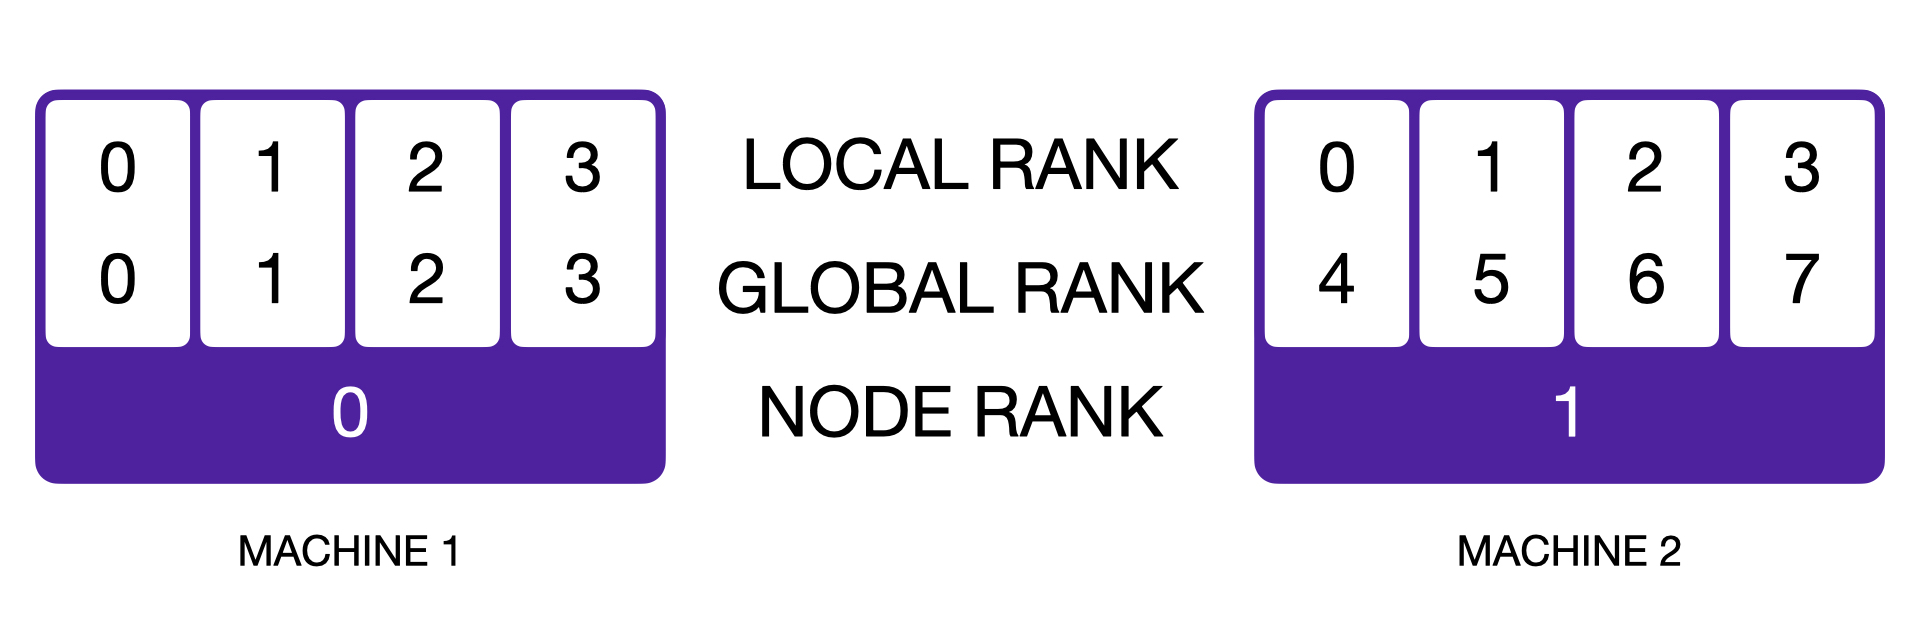
\includegraphics[width=0.95\textwidth]{figures/p32_r46.png}
\caption{运行在 2 个节点上、world size 为 8 的分布式应用示意图。每个工作进程由一个 global rank（0 到 7）和一个 local rank（0 到 3）标识。图取自 \url{https://lightning.ai/docs/fabric/stable/advanced/distributed_communication.html}}
\end{figure}

\subsubsection{分布式应用基准测试的最佳实践}

在作业的这一部分，你将对分布式应用进行基准测试，以更好地理解通信带来的开销。以下是一些最佳实践：

\begin{itemize}
  \item 只要有可能，就在同一台机器上运行基准测试，以便进行受控的比较。
  \item 在对目标运算计时之前，先进行若干次预热（warm-up）。这对 NCCL 通信调用尤其重要。通常 5 次预热迭代就足够了。
  \item 在 GPU 上做基准测试时，调用 \tm{torch.cuda.synchronize()} 等待 CUDA 操作完成。注意，即使调用带 \tm{async\_op=False} 的通信操作也需要这样做：该调用在操作被排入 GPU 队列时就会返回（而不是在通信实际完成时）。\footnote{更多细节见 \url{https://github.com/pytorch/pytorch/issues/68112\#issuecomment-965932386}。}
  \item 不同 rank 上的计时结果可能略有差异，因此通常要跨 rank 聚合测量结果，以改进估计。你会发现 all-gather 集合通信操作（具体来说是 \tm{dist.all\_gather\_object} 函数）对收集所有 rank 的结果很有用。
  \item 一般而言，先在本地用 Gloo 在 CPU 上调试，然后按照题目要求在 GPU 上用 NCCL 做基准测试。
\end{itemize}

在后端之间切换应当很简单：只需修改你的 \tm{init\_process\_group} 调用和张量设备转换即可。

\subsubsection*{问题（\tm{distributed\_communication\_single\_node}）：分布式通信（单节点）（5 分）}

编写一个脚本，对单节点多进程设置下 all-reduce 操作的运行时间进行基准测试。上面的示例代码可以作为一个合理的起点。尝试改变以下设置进行实验：

\begin{description}
  \item[all-reduce 数据大小] float32 数据张量，在 1MB、10MB、100MB、1GB 中取值。
  \item[GPU/进程数量] 2、4 或 6。
\end{description}

资源要求：最多 6 块 GPU。每次基准测试运行耗时应少于 5 分钟。

\textbf{交付物：}比较多组设置的图和/或表格，并附上 2-3 句话，评述你的结果以及你对这些因素之间如何相互影响的思考。
